\section{Empirical Evaluation}
\label{sec:experiments}
We evaluate three questions: how accurately endpoints can be estimated, how selective
observation changes model assessment, and which additional labels reduce unresolved
ambiguity. Simulated populations provide exact identification targets. Historical
applications test the consequences of changing the evaluation population. Controlled masking
of known outcomes permits direct checks of estimated risks and audit performance.
Appendix~\ref{app:experiments} provides the complete methods, results, and figure
provenance.

\subsection{Identification versus statistical uncertainty}
\label{sec:empirical-uncertainty}
We separate statistical uncertainty from population ambiguity in finite-cell populations
with Brier loss $\ell(f(x),y)=(f(x)-y)^2$, $\Gamma=2$, and $\alpha=.75$. An oracle
certificate uses the true outcome probability $p_1$ among historically observed cases and a
finite-cell Hoeffding radius. On the same sampled datasets, two-fold cross-fitting learns
the nuisance functions; root-mean-square error (RMSE) assesses the resulting endpoint
estimates. Each sample size uses 60 simulated populations and 80 datasets per population.

As $n$ increases from $10^3$ to $10^5$, mean oracle outer width falls from .614 to .147,
while mean exact population width remains .0949 (Figure~\ref{fig:finite-sample}a). The 95\%
oracle certificate contains the entire sharp interval in every replication; its simultaneous
protection across thresholds is conservative. Upper- and lower-endpoint RMSE decrease from
.0361 and .0425 to .0027 and .0023 (panel b). Larger samples sharpen estimation of the
interval, while the original observation process leaves its identification width intact. The
learned-nuisance experiment measures endpoint accuracy; coverage for learned fits requires
the calibration conditions of Theorem~\ref{thm:learning}.
Appendix~\ref{app:finite-sample-experiments} also reports the separate learning-bound
scaling diagnostic.

\begin{figure}[t]
\centering
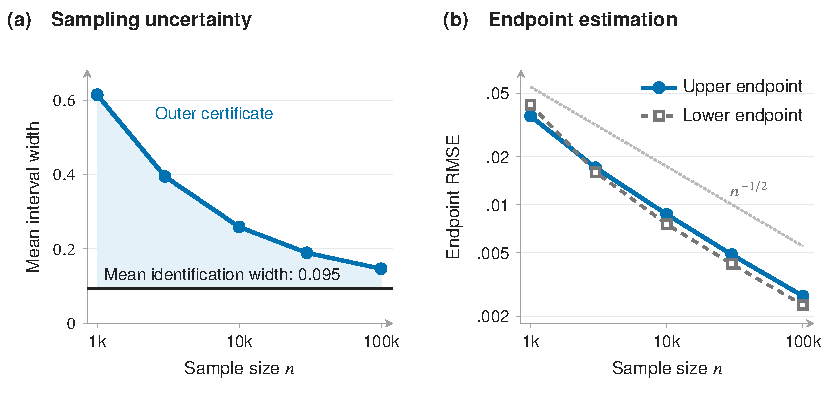
\includegraphics[width=\textwidth]{figures/fig02_learning.pdf}
\caption{\textbf{Statistical uncertainty contracts around an identification floor.} (a) Mean
oracle-calibrated outer width and mean exact population width; shading shows their
difference. (b) Cross-fitted endpoint RMSE with learned nuisances; the faint line is an
$n^{-1/2}$ guide. Each sample size uses 60 simulated populations and 80 datasets per
population. The oracle coverage target is the entire sharp interval.
Appendix~\ref{app:finite-sample-experiments} gives the design and complete results.}
\label{fig:finite-sample}
\end{figure}

\subsection{Historical applicant-level sensitivity analysis}
\label{sec:historical}
The 2012 LendingClub cohort contains 390,644 applications, including 53,367 mature issued
loans with known repayment outcomes \citep{george2019lendingclub}. The applicant target is
default under loan issuance; this outcome is unavailable for rejected applicants. The cohort
includes 180,903 applications with recorded credit-score values below 660, the 2012 FICO
minimum \citep{lendingclub2012registration}, and no issued loans in that group. We therefore
specify an issued-loan outcome regression extended to all recorded applicant covariates. Its
predictions supply the reference probabilities in \eqref{eq:robust-score}, together with the
observed-residual correction. The historical results are residual-adjusted sensitivity
estimates under this regression extension. Appendix~\ref{app:historical-lending} documents
unsupported regions and differences in how source fields were measured.

We compare logistic regression, default-weighted logistic regression, and gradient boosting
with five-fold cross-fitting. Default examples receive weight 2 in the weighted model.
Standard classification objectives represent existing prediction pipelines whose population
tail risks must be assessed. Brier loss is bounded and makes both possible label losses
explicit. We assess tail levels $\alpha\in\{.90,.95\}$.

At $\alpha=.95$, accepted-only CVaR favors the default-weighted model (.661). At $\Gamma=1$,
its estimated applicant risk is .813, compared with .733 for boosting and .805 for logistic
regression: two of three pairwise orderings reverse. Figure~\ref{fig:lendingclub}a gives the
intervals at $\Gamma=2$; Appendix~\ref{app:historical-lending} reports complete sensitivity
curves and approximate breakdown values.

The constant forecast $f\equiv1/2$ has loss $1/4$ under either label. Its mean Brier loss
and every CVaR therefore equal $1/4$, while identification width and TIV are zero. Its tail
loss is below that of the reported fitted models. Table~\ref{tab:sequential-performance}
shows the competing mean-loss advantage of the audited boosting models, whose mean Brier
losses are near .135. The reference separates average prediction quality, extreme-tail loss,
and certainty about that loss.

\subsection{Validation with known repayment outcomes}
\label{sec:known-outcomes}
We impose 20 outcome-dependent masks on the mature issued loans, with sensitivity
$\Gamma_0=3$ and approximately 45\% of labels observed. This study targets the issued-loan
reference population. Predictors are trained on observed labels using five-fold
cross-fitting, and their full-outcome CVaRs provide reference risks.

At $\Gamma_0$, plug-in intervals---the estimated endpoint intervals before statistical
widening---contain reference CVaR in 11--14 of 20 masks per predictor and tail level.
Enlargement using variability across five fold-specific objectives raises coverage to 19--20
(Figure~\ref{fig:lendingclub}b). Coverage here targets the full-outcome reference CVaR of
each fitted predictor. Fold enlargement provides an empirical calibration diagnostic.
Plug-in coverage is zero at every tested $\Gamma\le2$.

Three unordered predictor pairs in each of 20 masks give 60 comparisons per tail level. At
$\Gamma=3$, $\alpha=.95$, strict interval separation resolves 37 pairs correctly and leaves
23 unresolved. At $\Gamma=1$, the rule declares all 120 orderings across both tail levels
and makes 16 errors. Allowing the masking sensitivity changes both the inferred ordering and
whether separation supports a decision. Appendix~\ref{app:controlled-masking} gives the
mechanism, enlargement rule, and complete results.

\begin{figure}[t]
\centering
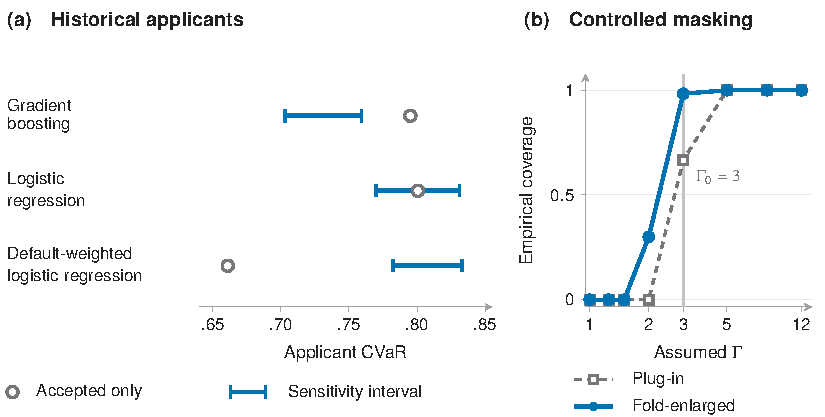
\includegraphics[width=\textwidth]{figures/fig03_assessment.pdf}
\caption{\textbf{Observation and sensitivity change population assessment.} (a) Accepted-only CVaR
(hollow points) and estimated applicant sensitivity endpoints (blue segments) at
$\alpha=.95$, $\Gamma=2$, under the regression extension of
Appendix~\ref{app:historical-lending}. Segments precede statistical enlargement. (b)
Coverage of full-outcome reference CVaR under controlled masking of mature issued loans, pooled across three
predictors and 20 shared masks at $\alpha=.95$. The guide marks the masking mechanism's
sensitivity $\Gamma_0=3$; fold enlargement is empirical.
Appendix~\ref{app:controlled-masking} provides the complete results.}
\label{fig:lendingclub}
\end{figure}

\subsection{Fixed and sequential audits}
\label{sec:empirical-revelation}
In 120 synthetic finite-cell populations with heterogeneous costs, TIV per cost matches the
exact fractional-knapsack frontier for fixed predictor and threshold
(Appendix~\ref{app:frontier-experiments}). We then audit the masked issued-loan population
using boosting, $\alpha=.95$, $\Gamma=3$, and unit cost per hidden label.

The fixed protocol freezes the initial predictor, historical nuisance estimates, and
upper-endpoint threshold. Newly audited outcomes become known contributions, while the
original sensitivity bounds remain on unaudited outcomes. The sequential protocol retrains
the predictor and reoptimizes thresholds after each batch; retained evaluation keeps the
historical outcome fit fixed, and a reserved split measures predictive loss. The
lowest-propensity baseline selects cases with the lowest estimated label availability; it
uses historical availability in the fixed protocol and refitted current known-label
availability in the sequential protocol.

At the recorded budget of approximately 16\%, TIV removes a median 61\% of the initial
estimated fixed-threshold gap, compared with 16\% for random acquisition
(Figure~\ref{fig:revelation-results}a). This concentration of removable ambiguity explains
the gain from targeting. For Brier loss, predictions near .5 have similar losses under
either label, so uncertainty sampling can favor cases with small excess-loss contrasts and
little identification value.

With sequential retraining, median estimated retained width falls from .097 to .035 under
TIV (panel b). This width describes the current predictor; it can increase when retraining
changes the assessed losses, as the other trajectories illustrate
(Table~\ref{tab:audit-protocols}). Terminal median held-out CVaR is .8541 for TIV and .8682
for random, while mean Brier loss is .1362 and .1347, respectively
(Table~\ref{tab:sequential-performance}). Relative to random acquisition, these runs show
improved tail performance and precision alongside a small mean-loss trade-off.
Appendix~\ref{app:repayment-audits} gives all policies and both protocols.

\begin{figure}[t]
\centering
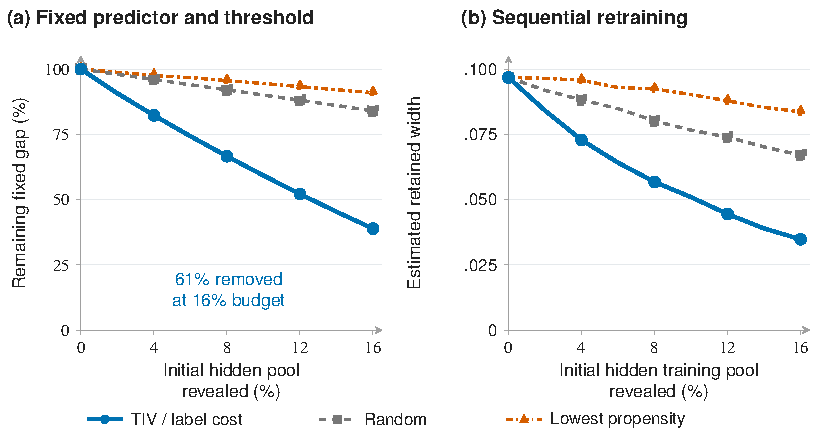
\includegraphics[width=\textwidth]{figures/fig04_revelation.pdf}
\caption{\textbf{Targeted audits reduce estimated ambiguity at equal within-protocol budgets.} (a)
Median remaining fixed-threshold gap, normalized within each mask by its initial estimated
gap. (b) Median estimated retained-sensitivity width for the predictor refitted after each
audit batch. Both use boosting, $\alpha=.95$, $\Gamma=3$, unit hidden-label cost, and 20
masks. Lines join eight recorded batches. Appendix~\ref{app:repayment-audits} specifies both
protocols. Budgets are median fractions of the initially hidden cases in each eligible pool: the original pool in (a) and the 80\% training pool in (b).}
\label{fig:revelation-results}
\end{figure}
